\chapter{Vorgehen Performance Analyse}
\section{Motivation}

Die Performance respektive Leistungsfähigkeit einer Applikation stellt einer der bedeutendsten Qualitätsanforderungen dar. Sie kann bei den Benutzern nicht nur zur Verärgerung, sondern auch zu einer Verlangsamung der Business-Prozesse führen. Die Motivation für eine Performance-Analyse entsteht, wenn die in Service Level Agreement oder Anforderungsanalyse spezifizierten \textbf{Qualitätsanforderungen nicht erfüllt} sind. Optimalerweise ist die Überprüfung dieser Anforderungen Bestandteil ein jedes Software Entwicklungszyklus respektive des (automatisierten) Testprozesses.

\section{Ablauf}
Die Performance-Analyse ist grundsätzlich ein iterativer Prozess und so lange bis die Anforderungen und der Kunde zufrieden sind. Sie besteht aus folgenden vier Schritten\cite{hummelBeer201109}:
\begin{enumerate}
	\item Identifikation der neuralgischen Punkte des Systems
	\item \textbf{Suche nach dem Dominating Consumer\footnote{Kirk Pepperdine bezeichnet die Aktivität, welche dominiert wie die CPU gebraucht wird, als Dominating Consumer . }}
	\item \textbf{Sammeln von Detaildaten}
	\item Lösen des Problems
\end{enumerate}

Punkt zwei und drei sind weiter unten weiter beschrieben.

\section{Suche nach dem Dominating Consumer}
Die Suche nach dem Dominating Consumer kann nach folgendem strukturierten Schema gemacht werden:
\begin{figure}[H]
  	\centering
    	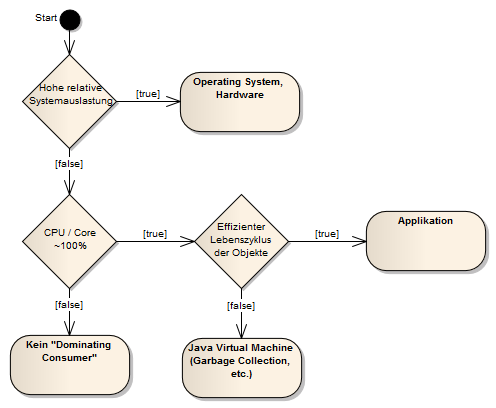
\includegraphics[width=13.1cm]{images/dominating_consumer}
        	\caption{Suche nach dem Dominating Consumer}
\end{figure}



\section{Sammeln von Detaildaten}

